\section{Projektinitialisierung}\label{sec:Projektinitialisierung}

\subsection{Unternehmen}

Wir sind ein junges Unternehmen bestehend aus drei Studenten der Sozialinformatik. Wir setzen uns zusammen aus zwei Softwareentwicklern (Backend- und Frontendentwickler) und einem Netzwerkadministrator. Das Unternehmen wurde im Jahr 2018 im Zuge eines IT"=Projekts für unser Studium gegründet.


\subsection{Projekt}

Die freiwillige Feuerwehr von Eschenstruth verwaltet die Feuerwehrkleidung für den eigenen, sowie die anliegenden Ortsteile Helsas. Dies gestaltet sich zunehmend schwerer, da die aktuelle Bestandspflege und der Überblick über die ausgegebene Kleidung mit den aktuellen Methoden sehr fehleranfällig und unübersichtlich ist. Vor wenigen Jahren wurden die Ausgabe und Verwaltung der Kleidung noch mit Zetteln dokumentiert. Dabei kam es durch uneinheitliches Vorgehen zu Verlust von Informationen. Dies geschah \zb durch den Verlust eines Zettels. Ein Zettel konnte schnell geschrieben, musste aber auch ordentlich in die entsprechende Akte eingepflegt werden. Zudem musste der Ort der Akte erst aufgesucht werden um das Schriftstück abzuheften.
Aktuell wird eine Excel"=Tabelle gepflegt. Diese befindet sich auf einem lokalen Rechner und einem USB"=Stick zur Datensicherung. Hier besteht der Nachteil, dass ein Rechner, auf dem sich de Excel"=Tabelle befindet, aufgesucht werden muss, um den Kleidereingang oder "=ausgang aus dem Lager zu dokumentieren. Als Zwischenspeicher wird eine Tafel verwendet, die bei der Ausgabe oder Annahme von Kleidung gefüllt wird (s. Abbildung~\ref{fig:tafel}). Der Warenbestand kann dann von einem beliebigen Rechner aus übertragen und dokumentiert werden, unter der Voraussetzung, dass die Person die aktuelle Excel"=Tabelle besitzt. Es muss aber bei der Synchronisation der Dokumentation darauf geachtet werden, dass die Daten in chronologisch richtiger Reihenfolge aufbereitet werden. Das kann unter Umständen, wenn zwei Personen zur gleichen Zeit an der Tabelle gearbeitet haben, zu einem erheblichen Mehraufwand führen, wenn nicht direkt nachvollziehbar ist, wer als letztes die Tabelle gepflegt hat, oder auf welchen Stand sich die Excel"=Tabelle befindet. 

\begin{figure}[hbtp]
  \centering
  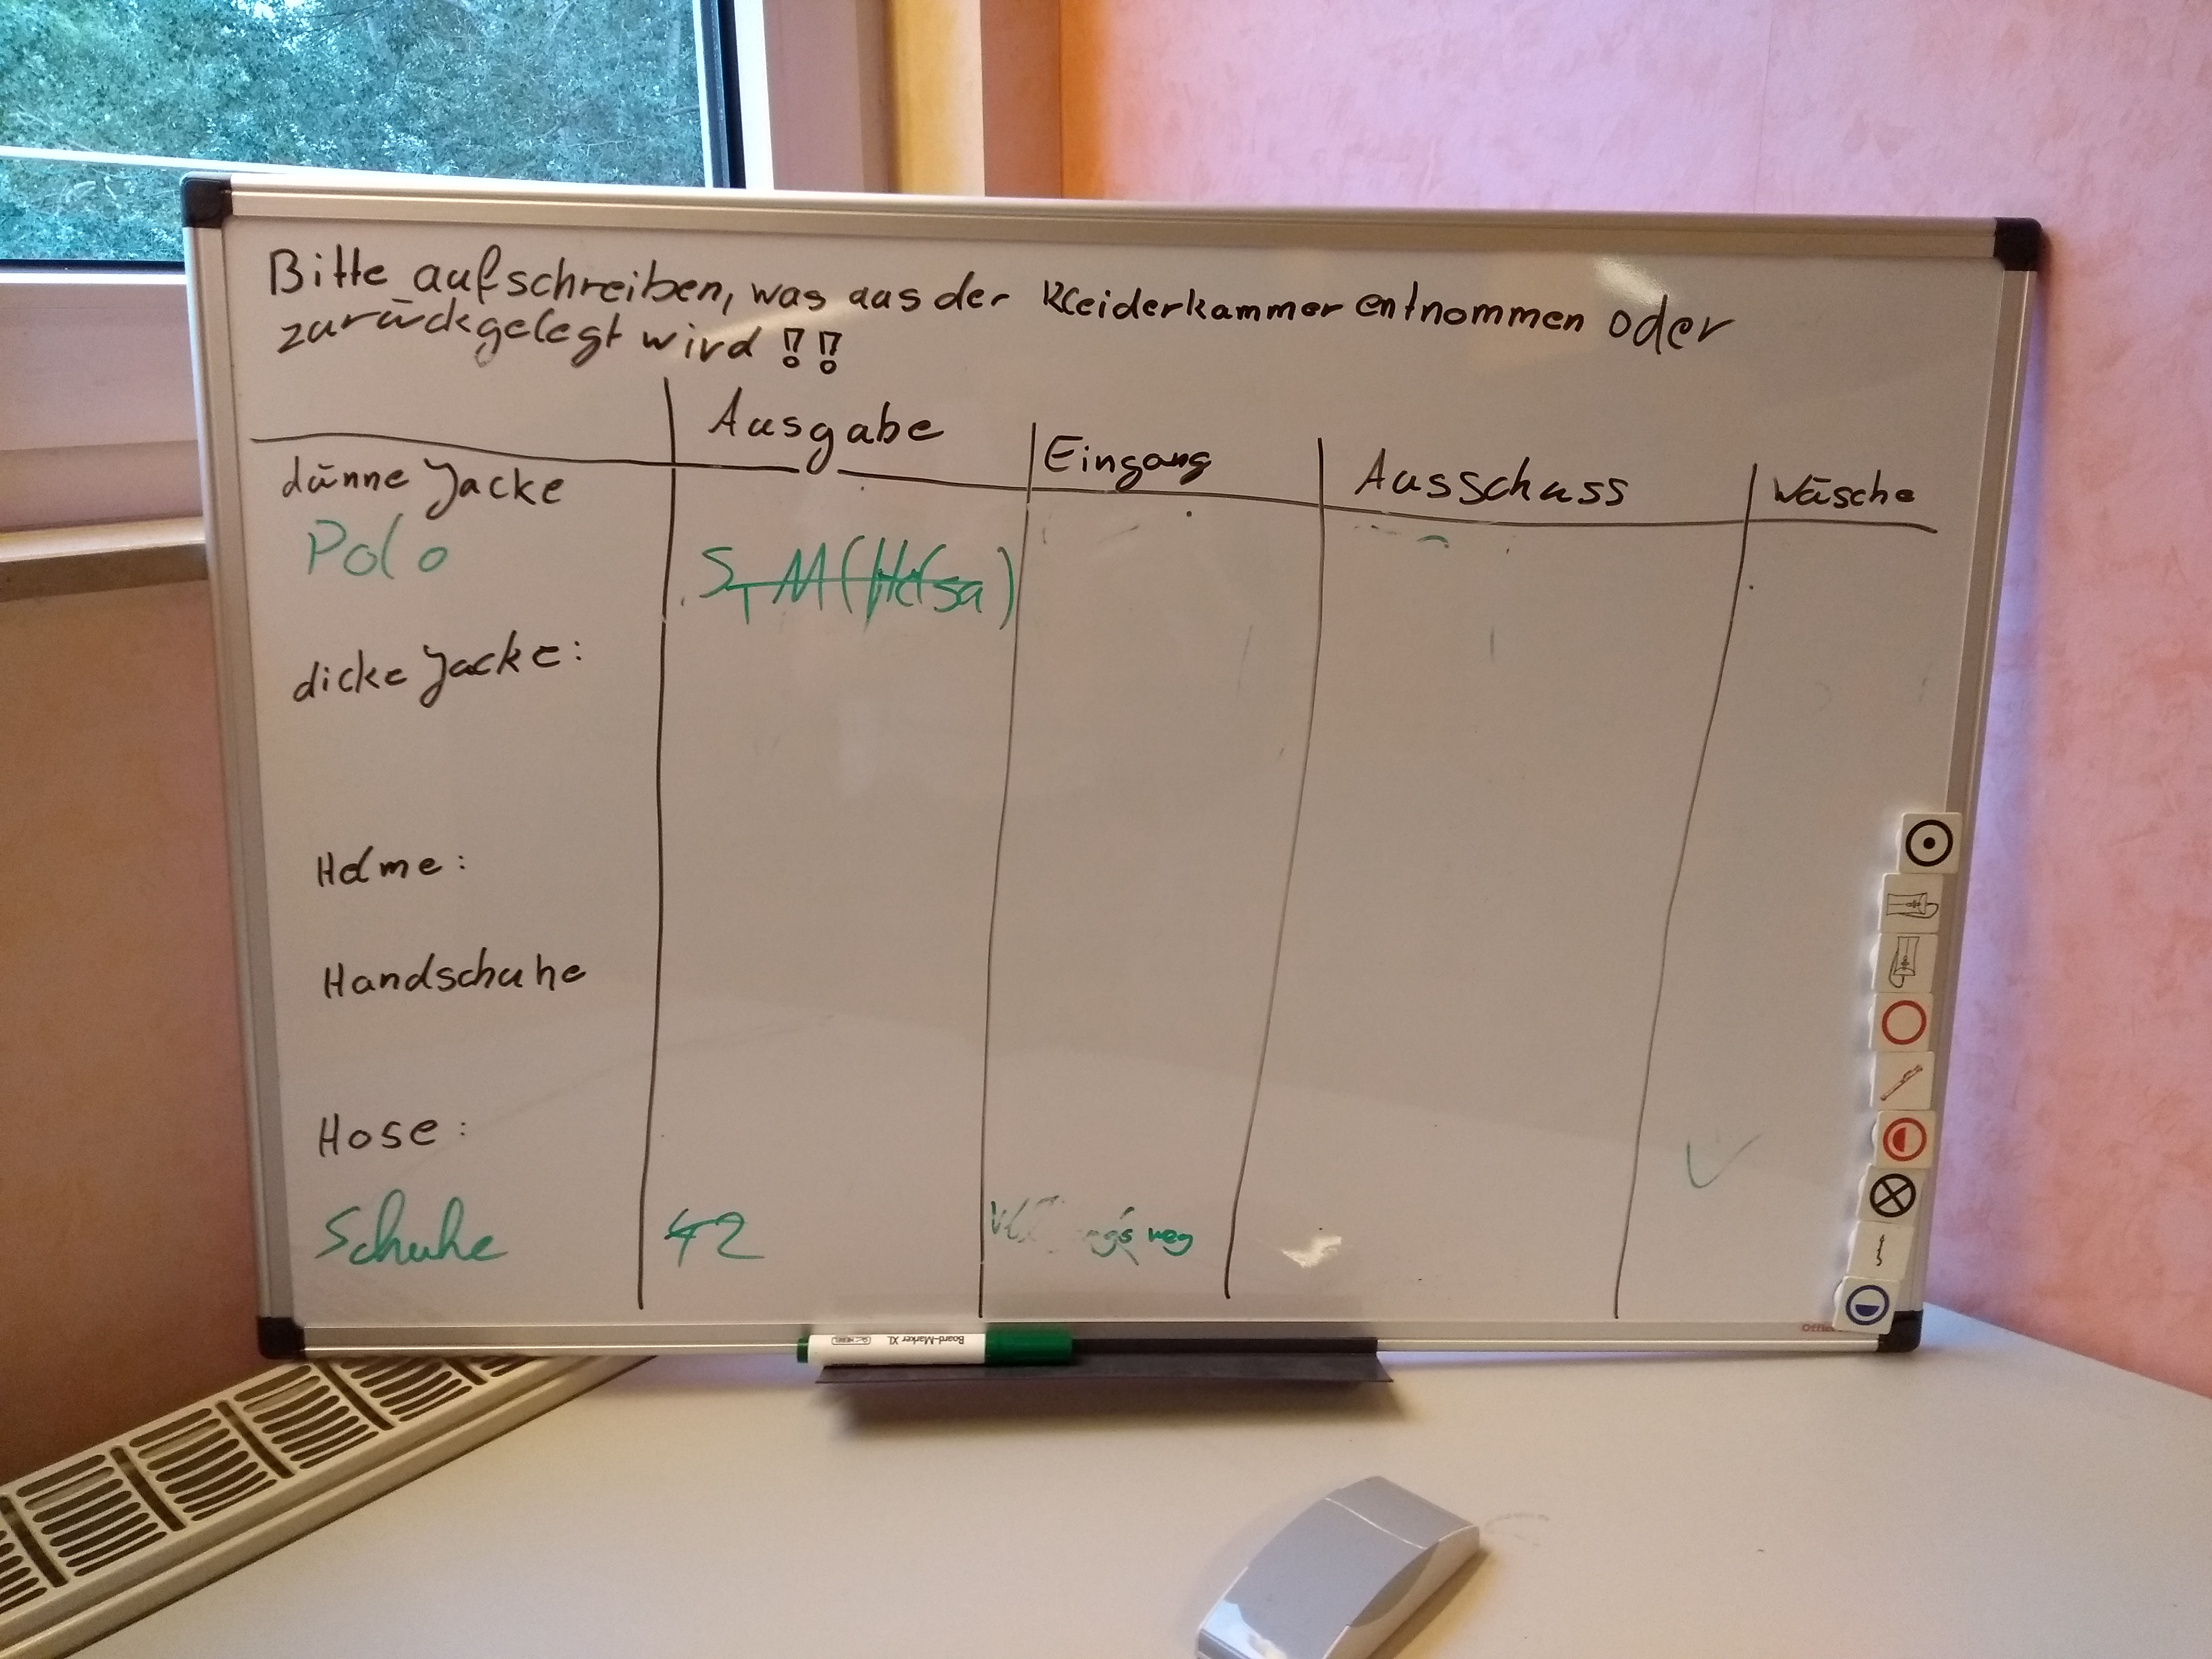
\includegraphics[width=0.95\textwidth]{res/IMG_20180815_193814370}
  \caption{Tafel aus Zwischenspeicher von Informationen.}
  \label{fig:tafel}
\end{figure}

Um die Probleme des Datenverlusts und der Synchronisation von Daten zu beseitigen, kam die Idee einer zentralen, aus dem Internet erreichbaren Kleiderverwaltung der Jugendfeuerwehr von Eschenstruth, oder auch \project, auf.

In den folgenden Kapiteln werden die Kernziele dieses Projekts erläutert und die Erfolgskriterien definiert. Die beteiligten Personen an diesen Projekt werden erfasst und kurz vorgestellt. Darauf folgt der Projektansatz mit der Anforderungsspezifikation. Dabei werden alle Anforderungen die zwingend in diesem Projekt umgesetzt werden müssen definiert. 

\subsection{Project Definition Document}

\subsubsection{Gegenstand, Kernziele und Ziele des Projektes}

Unsere Kernziele sind das Schaffen einer Übersicht über die Bestände der Kleidung der Jugendfeuerwehren der Gemeinde Helsa. Diese werden aktuell im Ortsteil Eschenstruth gelagert und rudimentär verwaltet. Dafür soll eine Web"=Applikation erstellt werden, die den Bestand dokumentiert, sowie die Aus"= und Abgabe von Kleidung der freiwilligen Feuerwehr Helsa Ortsteil Eschenstruth ermöglicht. 

Das Projekt soll möglichst barrierefrei (nach aktuellstem europäischem Standard), sowie mobil bedienbar sein, sodass die Jugendwarte nicht auf einen zusätzlichen Laptop angewiesen sind, sondern das Programm einfach und bequem von ihrem Laptop oder Smartphone aus bedienen können. Es soll außerdem unter Verwendung der aktuellsten technischen Standards umgesetzt werden.

Ziel ist es eine vollständig nachvollziehbare Dokumentation zu ermöglichen, bei der zu jederzeit der aktuelle Aufenthaltsort der zur Verfügung stehenden Kleidung ermittelt werden kann. Dabei soll ein paralleles Arbeiten möglich sein. 

\subsubsection{Erfolgskriterien}

Wir sind sehr darauf bedacht, eine performante und jederzeit erreichbare Applikation zu entwickeln. Ein schneller Seitenaufbau und kurze Wartezeiten sind serhr wichtig , da sie die Akzeptanz der Anwender steigern werden. Hierfür ist uns eine gute Server-Infrastruktur wichtig.

Wir legen außerdem gesteigerten Wert darauf, dass die Anwendung mobil nutzbar sein wird. Das soll zum einen ebenfalls die Akzeptanz der Anwender steigern und zum anderen das Anschaffen neuer Hardware verhindern.

Ein weiteres Erfolgskriterium ist die vollständige Ablösung der Excel"=Tabelle und der Tafel. Die Daten werden nur noch über die Anwendung gepflegt.


\subsubsection{Kontext des Projektes und die Projektabhängigkeiten}

Unser Projekt wird im Kontext unseres Studiums der Sozialinformatik umgesetzt. 
Das Projekt soll für einen öffentlichen, sozialen Träger umgesetzt werden: Die freiwillige Feuerwehr der Gemeinde Helsa, oder spezifisch des Ortsteiles Eschenstruth. Dort sind nur ehrenamtliche Kräfte tätig, die dafür sorgen, dass der Brandschutz in der Gemeinde Helsa und für den neuen Autobahnabschnitt der A44 zwischen Kassel und Hessisch-Lichtenau gewährleistet werden kann. 

\subsubsection{Risiken, die den Projekterfolg verhindern könnten}

Dadurch, dass das Projekt"=Team Vollzeit tätig ist, kann es zu Engpässen in der Durchführung kommen. Dies kann unter Umständen zu Mehrarbeit auf einzelne Team"=Mitglieder führen. Das Risiko ist gering einzuschätzen, da das Projekt"=Team  hinter der Idee steht.

Ein weiteres Risiko betrifft die Evaluation einer kostenlosen, bis kostengünstigen, Plattform, auf der die Anwendung bereit gestellt werden kann. Dabei kann die Akzeptanz der Endkunden sinken, wenn die Betriebskosten zu hoch ausfallen. Ab welchen Betrag die Kosten zu hoch sind, ist noch zu klären. Dieses Risiko ist mittelmäßig einzuschätzen, da es am Markt diverse Anbieter gibt. Unter den bekannteren Anbietern gehören \textit{AWS}, von \textit{Amazon}, sowie \textit{Heroku}.

\subsubsection{Am Projekt Beteiligte}\label{sec:beteiligte}

Zum Projekt"=Team gehören:

\begin{itemize}
\item Tim Wieder, ist zuständig für den Kundenkontakt und die Frontend"=Entwicklung.
\item Achim Rose, ist zuständig für die Backend"=Entwicklung und den Entwurf der Datenbanktabellen. 
\item Sebastian Seeger, ist zuständig für die Infrastruktur. Das betrifft die Evaluation der Plattform und dessen Konfiguration.
\end{itemize}

Zu den Kunden, sprich die Beteiligten der freiwilligen Feuerwehr Eschenstruth, gehören: 

\begin{itemize}
\item Nico M. (zuständig für die Kleiderkammer)
\item Julia W.
\item Marcel B.
\item Markus N.
\item Florian B.
\item Philipp H.
\end{itemize}

\subsubsection{Zu erwartender Projektansatz}

Das Projekt wird mit dem agilen Softwareentwicklungsframework \textit{Scrum} umgesetzt. Der Vorteil hierbei ist die Freiheit für die Entwickler, die sich die Arbeit so einteilen können, wie es für sie gerade passend ist. Dabei werden regelmäßig \textit{Dailys} abgehalten, um die anderen Projektteilnehmer auf den aktuellen Entwicklungsstand zu bringen.

\newpage
